\chapter{مقدمه}
\clearpage

در سال‌های اخیر، با افزایش جمعیت سالمندان، فشارها بر روی مراکز بهداشتی و مراقبتی افزایش یافته است. این امر علاوه بر افزایش هزینه‌ها، می‌تواند باعث شود که نیروی انسانی نتواند به خوبی وظایف خود در مراقبت از افراد را به دلایل مختلفی مانند خستگی و یا فراموشی ایفا کند. به همین دلیل به سیستم‌های هوشمند مراقبتی نیاز داریم تا بتوانند بهتر و با هزینه‌ی کمتر و بهینه‌تری وظیفه‌ی مراقبت از افراد کم‌توان را انجام دهند. وجود سیستم‌های هوشمند باعث می‌شود که سالمندان بدون نیاز به داشتن کمک از جانب افراد مختلف، بتوانند زندگی مستقل و در عین حال با کیفیتی را داشته باشند.

پیشرفت‌ها در حوزه‌های متعدد فناوری مانند افزایش قدرت پردازشی ریزپردازنده‌ها، کاهش هزینه‌ی تولید و بهبود کیفیت خروجی حسگرها امکان ایجاد همچین سیستم‌هایی را ممکن کرده است. وظیفه‌ی کلی این سیستم‌ها این است که فعالیت افراد تحت مراقبت را در لحظه شناسایی کنند و در صورت لزوم به آن‌ها کمک کنند. به‌طور کلی فرایند شناسایی فعالیت‌های انسانی در بسیاری از موارد مانند خانه‌های هوشمند\cite{alaghbari2022activities,liao2014detecting}،
بازی‌ها\cite{almeida2017activity}،
محاسبات شهری\cite{zambonelli2011pervasive}،
روباتیک\cite{pereyda2019cyber}،
پیش‌بینی فعالیت بعدی\LTRfootnote{Next Activity Prediction}\cite{alaghbari2022activities,jaouedi2020prediction}،
تشخیص ناهنجاری\LTRfootnote{Anomaly Detection}\cite{alaghbari2022activities,zhu2015wearable}
و اینترنت اشیا (\verb;IoT;\LTRfootnote{Internet of Things})\cite{lu2018wearable}
کاربردهای بسیاری داشته‌اند و نتایج خوب و امیدوار کننده‌ای را از خود نشان داده‌اند.

روش‌های شناسایی فعالیت انسان\LTRfootnote{Human Activity Recognition}
را از روی نوع داده‌ی مورد استفاده می‌توان به دو دسته تقسیم کرد. دسته‌ی اول، شامل استفاده از داده‌های دوربین‌ها و پردازش تصویر و دسته‌ی دوم، شامل استفاده از داده‌های انواع حسگرها می‌باشد.

استفاده از داده‌های دوربین و تصاویر در محیط‌های عمومی کاربرد دارد. با استفاده از داده‌های دوربین به‌ویژه داده‌های دنباله‌ای از تصاویر به‌صورت پیوسته (مانند یک فیلم) می‌توان تعدادی
فعالیت ابتدایی\LTRfootnote{Action Primitive}
مانند جهت حرکت دست را کشف کرد و سپس با ترکیب این فعالیت‌ها، به عمل انجام شده توسط شخص پی برد\cite{dhillon2017recent}.
اما نکته‌ای که در رابطه با داده‌های تصویری وجود دارد این است که به دلایل مربوط به حریم شخصی، نمی‌توان از این داده‌ها برای هوشمندسازی شناسایی فعالیت در تمامی محیط‌ها، به‌ویژه خانه‌ها استفاده کرد چرا که ذخیره‌سازی اطلاعات تصاویر و پردازش آن‌ها حریم خصوصی افراد را مختل خواهد کرد. علاوه بر آن، دوربین‌ها نقاط کور دارند و برای عملکرد خوب دوربین‌ها نیاز داریم که در تمامی نقاط خانه دوربین قرار دهیم. اما این امر میسر نیست؛ چرا که علاوه بر هزینه‌ی زیاد قرار دادن تعداد زیادی دوربین در تمامی نقاط خانه، در تعدادی از نقاط خانه مانند حمام امکان قرار دادن دوربین وجود ندارد و در صورت رخ دادن هر گونه اتفاق غیر منتظره‌ای برای افراد تحت مراقبت در این محیط‌ها امکان شناسایی این امر وجود ندارد و خطرات جانی را به همراه خواهد داشت. به همین دلیل علیرغم عملکرد خوب روش‌های شناسایی فعالیت بر مبنای
داده‌های تصویری\cite{mathew2023human}،
بهتر است که از روش‌هایی برای شناسایی فعالیت استفاده کنیم که قابل استفاده در انواع محیط‌های هوشمند، به‌ویژه خانه‌ها که افراد (به‌خصوص سالمندان) زمان زیادی از روز را در آن سپری می‌کنند، باشد.

به همین دلیل به روش‌های شناسایی فعالیت مبتنی بر داده‌های حسگرها روی می‌آوریم. روش‌های مبتنی بر داده‌های حسگر، خروجی یک یا مجموعه‌ای از حسگرها را به عنوان داده‌ی ورودی در نظر می‌گیرند و بر روی آن‌ها پردازش انجام می‌دهند. حسگرهای مورد استفاده می‌توانند از نوع
محیطی\LTRfootnote{Ambient Sensors}\cite{cook2012casas}،
پوشیدنی\LTRfootnote{Wearable Sensors}\cite{vavoulas2016mobiact}
و یا هر دو\cite{roggen2010walk}
باشند. وظیفه‌ی حسگرهای محیطی اندازه‌گیری تغییرات در محیط مانند لمس اجسام مختلف، تغییرات دما و مجاورت اجسام می‌باشد. از طرفی حسگرهای پوشیدنی تحرکات کاربر را با دقت بهتری می‌توانند بررسی کنند و جزئیات بهتری از نحوه و جهت حرکت کاربر را به ما بدهند. حسگرهای حرکتی
شتاب‌سنج\LTRfootnote{Accelerometer}،
ژیروسکوپ\LTRfootnote{Gyroscope}
و لَختی (اینرسی\LTRfootnote{Inertia})
از جمله حسگرهای پوشیدنی می‌باشند. علاوه بر آن، امروزه به دلیل پیشرفته شدن تلفن‌های همراه، می‌توان به سادگی از یک تلفن همراه بعنوان انواع حسگرهای پوشیدنی به‌طور همزمان استفاده کرد\cite{reyes2016transition}؛
و با توجه به این که در عصر حاضر کمتر کسی از تلفن‌های همراه هوشمند استفاده نمی‌کند، به سادگی و با کمترین هزینه‌ی سخت‌افزاری می‌توان فعالیت اشخاص را شناسایی کرد.

یادگیری عمیق\LTRfootnote{Deep Learning}
به دلیل دقت بالایی که از خود نشان داده است\cite{chen2021deep}
(مانند حافظه کوتاه مدت بلند (\verb;LSTM;\LTRfootnote{Long Short-Term Memory}) و شبکه‌ی عصبی پیچشی\LTRfootnote{Convolutional Neural Network})،
به روش اصلی مسائل مربوط به شناسایی فعالیت انسان در سال‌های اخیر تبدیل شده است. این روش‌ها با بهره‌گیری از
توابع فعال‌ساز غیرخطی\LTRfootnote{Non-linear Activation Functions}
و الگوریتم پس‌انتشار خطا\LTRfootnote{Backpropagation Algorithm}\cite{rumelhart1986learning}
این امکان را فراهم می‌کنند که مدل‌های بسیار عمیق و دارای پارامترهای با تعداد بالا آموزش داده شوند که با انتخاب معماری مناسب و داده‌ی برچسب‌گذاری شده‌ی کافی، امکان کشف روابط پیچیده در داده‌ی ورودی را به شبکه‌های عصبی عمیق می‌دهد؛ بر خلاف روش‌های سنتی یادگیری ماشین که یا بدون پارامتر هستند (مانند روش \verb;K;-نزدیک‌ترین همسایه (\verb;KNN;\LTRfootnote{K-Nearest Neighbors}))
یا در صورت داشتن پارامتر، دارای تعداد پارامتر قابل یادگیری بسیار کمی هستند
(مانند روش رگرسیون لجستیک\LTRfootnote{Logistic Regression} که دارای تنها \verb|d+1| پارامتر هستند که \verb|d| بیانگر تعداد ابعاد ورودی است).
به همین دلیل شبکه‌های عصبی با داشتن تعداد زیادی پارامتر قابل یادگیری و پیچیدگی بالا، می‌توانند عملکرد خیلی خوبی نسبت به روش‌های سنتی یادگیری ماشین نشان دهند.

اما همانطور که اشاره کردیم، مدل‌های یادگیری عمیق
دارای نظارت\LTRfootnote{Supervised}
برای عملکرد خوب خود نیازمند حجم زیادی داده‌ی برچسب‌گذاری شده می‌باشند. در صورت کافی نبودن داده‌های آموزشی، عملکرد مدل افت خواهد کرد و مدل دچار
بیش‌برازش\LTRfootnote{Overfitting}
یا کم‌برازش\LTRfootnote{Underfitting}
(بسته به پیچیدگی مدل و پیچیدگی داده‌ها)
خواهد شد. علاوه بر آن، حتی هنگامی که داده‌های کافی برای آموزش داشته باشیم، مدل‌های یادگیری عمیق هنگامی عملکرد خوبی از خود نشان خواهند داد که توزیع آماری داده‌های آموزشی و ارزیابی شباهت زیادی با یکدیگر داشته باشند. در واقع
قدرت تعمیم\LTRfootnote{Generalization}
مدل‌های یادگیری عمیق دارای نظارت به‌طور کلی خیلی بالا نیست و در شرایطی که داده‌های ارزیابی شبیه به داده‌های آموزشی نباشند، این مدل‌ها افت عملکرد خواهند داشت\cite{recht2019imagenet}.
امری که در داده‌های دنیای واقعی کاملا مشهود است. بعنوان مثال در وظیفه‌ی شناسایی فعالیت انسان، داده‌ی حسگرها برای افراد سالمند و افراد جوان و کودکان و حتی افراد مختلف با سن و شرایط جسمانی یکسان تفاوت‌های بسیاری دارند چرا که نحوه‌ی انجام فعالیت‌ها توسط افراد مختلف متفاوت است و منجر به تولید داده‌ها از توزیع‌های متنوع می‌شود. همینطور با قرار دادن حسگر در نقاط مختلف بدن یا چرخش جهت حسگر (مثلا قرار دادن تلفن همراه در خلاف جهت قرار داده شده در مجموعه داده) توزیع داده‌های تولیدی توسط حسگرها می‌تواند تغییراتی کند که منجر به افت کیفیت مدل در تولید خروجی شود\cite{cleland2013optimal}.
\begin{figure}[htbp]
  \centering
  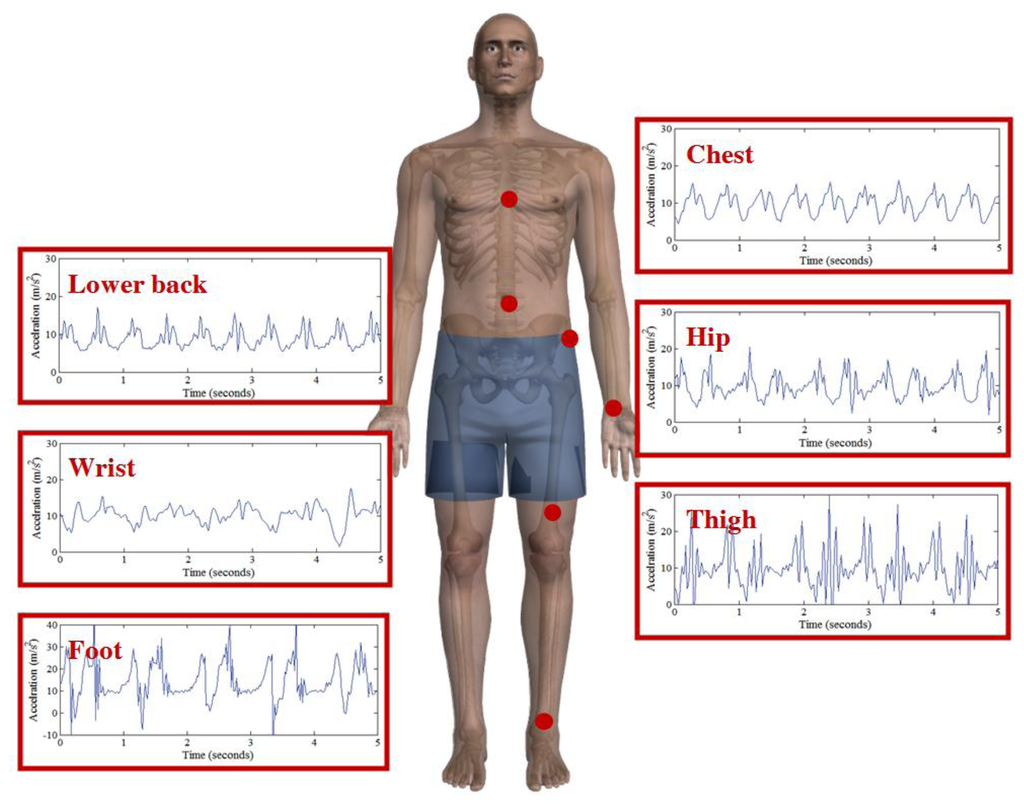
\includegraphics[width=0.8\textwidth]{Images/Chapter1/accelerometer-placement.png}
  \caption{تفاوت داده‌های تولیدی توسط حسگر شتاب‌سنج قرار گرفته در نقاط مختلف بدن}
  \label{fig:accelerometer-placement}
\end{figure}

علاوه بر مشکل تعمیم مدل بر روی داده‌های جدید، معضل برچسب‌گذاری داده‌ها نیز وجود دارد. چرا که برای برچسب‌گذاری داده‌های خام، نیاز به نیروی انسانی داریم. بعنوان مثال، مجموعه داده‌ی
\verb|ImageNet|
شامل 3.1 میلیون تصویر از 1000 کلاس مختلف می‌باشد که هر کدام از این تصاویر کاملا توسط نیروی انسانی برچسب خورده‌اند\cite{deng2009imagenet}.
طبیعتا برچسب‌گذاری این داده‌ها کاری بسیار طاقت‌فرسا و پرهزینه می‌باشد؛ اما برچسب‌گذاری داده‌های تصویری به مراتب ساده‌تر از برچسب‌گذاری داده‌های حسگرها می‌باشد. چرا که داده‌های تصویری برای افراد آشنا هستند و اشخاص می‌توانند با نگاه به تصاویر متوجه شوند که تصویر چه برچسبی را خواهد داشت. اما برای داده‌های حسگرها نمی‌توان صرفا از روی داده‌ی خام حسگر، فعالیت انجام شده‌ی مربوطه را به‌دست آورد. بنابراین برای برچسب‌گذاری داده‌ی حسگرها بایستی که یک متخصص در تمام مدت آزمایش حرکات شخص مورد آزمایش را زیر نظر بگیرد و برچسب‌گذاری کند. این امر باعث می‌شود که برای تولید حجم زیادی داده‌ی برچسب‌دار برای مسئله‌ی شناسایی فعالیت انسان، زمان و هزینه‌ی بسیار زیادی صرف شود و علاوه بر آن داده‌ها در محیط آزمایشگاهی که با دنیای واقعی متفاوت هستند تولید شوند.

به دلایلی که ذکر کردیم، نیاز به روش‌هایی داریم که وابستگی مدل‌ها را به داده‌های برچسب‌خورده کاهش دهیم و در عین حال قدرت تعمیم آن‌ها را افزایش دهیم. یکی از رویکردهای نوین برای رسیدن به این هدف، بهره‌گیری از یادگیری خودنظارتی\LTRfootnote{Self-Supervised Learning}
(که زیرمجموعه‌ای از یادگیری بدون نظارت\LTRfootnote{Unsupervised Learning} است)
می‌باشد. در این رویکرد، مدل با استفاده از ساختارهای درونی و الگوهای موجود در داده‌های بدون برچسب، پیش‌وظایفی را تحت عنوان
وظایف پوششی\LTRfootnote{Pretext tasks (Auxiliary tasks)}
اجرا می‌کند و مدل از آن‌ها برای یادگیری
بازنمایی\LTRfootnote{Representation}های
مفید بهره می‌برد. این پیش‌وظایف می‌تواند شامل مواردی مانند شناسایی چرخش\cite{gidaris2018unsupervised}،
روش‌های مبتنی بر ایجاد داده مانند تکمیل بخش‌های حذف شده از داده\cite{he2022masked}
و روش‌های مبتنی بر یادگیری تباینی\LTRfootnote{Contrastive Learning}\cite{chen2020simple,grill2020bootstrap,caron2020unsupervised}
باشد. همچنین در بسیاری از این روش‌ها، به‌منظور تقویت اثربخشی فرایند یادگیری، از تکنیک‌های
داده‌افزایی\LTRfootnote{Data Augmentation}
(مانند ایجاد نسخه‌های متغیر از یک نمونه‌ی داده با حفظ معنای کلی آن از طریق روش‌هایی مانند افزودن نویز و ایجاد برش بر روی داده‌ها) بهره گرفته می‌شود. با انجام این وظایف و حل این‌گونه مسائل، یک تابع هزینه نیز برای مدل تعریف می‌شود که مدل در طی فرایند کمینه کردن این تابع هزینه، بازنمایی‌های خوبی از داده یاد می‌گیرد که از وزن‌های تصادفی اولیه‌ی مدل عملکرد بسیار بهتری دارند.
سپس با استفاده از این بازنمایی‌ها می‌توانیم در مراحل بعدی برای حل وظایف دارای برچسب (مانند دسته‌بندی فعالیت‌ها) مدل را
تنظیم دقیق\LTRfootnote{Fine-tune}
کنیم و عملکرد قابل قبولی را حتی با حجم کمی از داده‌های برچسب‌خورده به‌دست آوریم\cite{gidaris2018unsupervised}.
استفاده از یادگیری خودنظارتی، نه تنها هزینه‌های مربوط به برچسب‌گذاری را به‌طور چشم‌گیری کاهش می‌دهد، بلکه با بهره‌گیری از حجم زیاد داده‌های بدون برچسب، قابلیت تعمیم مدل را نیز در مواجهه با داده‌هایی از توزیع‌های متفاوت افزایش می‌دهد. بدین صورت که می‌توانیم مدل را بر روی یک مجموعه داده‌ی بسیار بزرگ اما بدون برچسب پیش‌آموزش دهیم و سپس به‌وسیله‌ی
یادگیری انتقالی\LTRfootnote{Transfer Learning}،
بر روی مجموعه داده‌ی کوچک تنظیم دقیق انجام دهیم. تحقیقات نشان داده‌اند که پیش‌آموزش مدل به‌روش خودنظارتی و سپس تنظیم دقیق بر روی تنها بخش کوچکی از مجموعه داده‌ی مقصد
(یادگیری با نمونه‌ی اندک\LTRfootnote{Few-shot learning})،
عملکرد بهتری را نسبت به پیش‌آموزش به روش دارای نظارت نشان می‌دهد\cite{chen2020big,yuan2024self}.
این ویژگی به‌ویژه در مسئله‌ی شناسایی فعالیت انسان که در آن تنوع بالایی در نحوه‌ی انجام فعالیت وجود دارد و همچنین کوچک‌ترین تغییراتی مانند وجود حیوان خانگی می‌تواند عملکرد مدل را مختل کن، از اهمیت بالایی برخوردار است. از این‌رو، استفاده از یادگیری خودنظارتی به عنوان یک راهکار جایگزین یا مکمل یادگیری دارای نظارت گامی مؤثر در جهت ارتقاء کارایی مدل‌ها در شرایط دنیای واقعی برداشته است.

\section{دستاوردهای پژوهش}

دستاوردهای کلی این پژوهش شامل موارد زیر می‌شوند:

\begin{itemize}
\item{پیاده‌سازی یک رویکرد یادگیری خودنظارتی تباینی بر مبنای خوشه‌بندی\LTRfootnote{Clustering}}
\item{استفاده از تبدیل موجک\LTRfootnote{Wavelet Transform} برای بهره‌گیری از مولفه‌های فرکانسی داده}
\item{بهبود روش‌های تولید داده‌ی افزوده برای تبدیل موجک}
\item{آزمایش و ارزیابی مدل ارائه شده در یادگیری انتقالی}
\end{itemize}

\section{ساختار مطالب}
در این پایان‌نامه،‌ فصل دوم به مرور پیشینه پژوهش و روش‌هایی که تاکنون در حوزه شناسایی فعالیت انسان، یادگیری خودنظارتی و کاربردهای یادگیری خودنظارتی در شناسایی فعالیت انسان ارائه شده‌اند اختصاص دارد. فصل سوم به معرفی مدل پیشنهادی این پژوهش پرداخته و ساختار مدل، الگوریتم‌های به‌کاررفته و نحوه استفاده از آن‌ها بررسی می‌گردد. در فصل چهارم، نتایج حاصل از آزمایش‌های انجام‌شده با استفاده از روش پیشنهادی در مقایسه با روش پایه ارائه می‌گردد و با تحلیل این نتایج، فصل خاتمه می‌یابد. در نهایت،‌ فصل پنجم به جمع‌بندی و نتیجه‌گیری و ارائه‌ی پیشنهاداتی برای کارهای آینده اختصاص دارد.
